\chapter{Assignment \#3}
\label{ch:ass3n}

\begin{fullwidth}


%\begin{wrapfigure}{r}{0.4\textwidth}
%\centering
%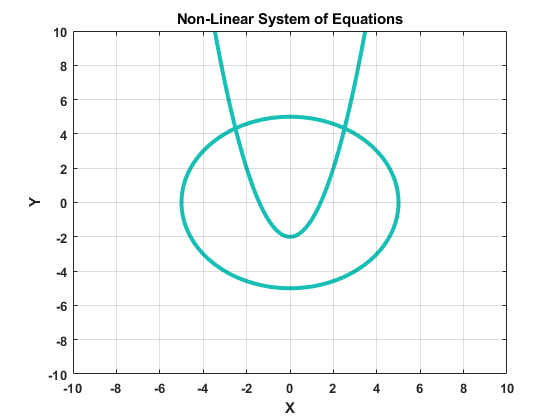
\includegraphics[width=0.35\textwidth]{ass3n_problem1_system.png}
%\caption{Non-linear system for problem \#1.}
%\label{fig:ass3n-prob1-system}
%\end{wrapfigure}




\begin{enumerate}

\item Consider a non-linear system of equations comprising the following functions:

%\begin{adjustbox}{minipage={\linewidth}, valign=t}
%\begin{wrapfigure}{t}{0.4\linewidth}
%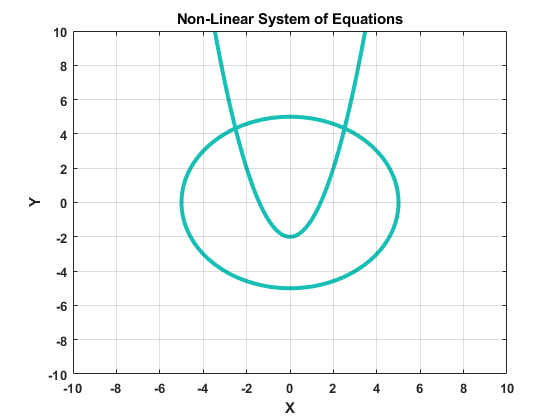
\includegraphics[width=\linewidth]{ass3n_problem1_system.png}
%\caption{Non-linear system for problem \#1.}
%\label{fig:ass3n-prob1-system}
%\vspace{-1.65\baselineskip}
%\end{wrapfigure}
%\vspace*{0.25em}
%\blindtext
%\end{adjustbox}

\begin{align*}
f(x,y) &= x^2 + y^2 - 25 = 0 \\
g(x,y) &= x^2 - y - 2 = 0
\end{align*}
Create a function to carry out Newton's method for finding a root for this system of non-linear equations.  The function should have the signature: \lstinline[style=myMatlab]{Xs = NewtonSystemSol(Fun, Jac, Xo, Tol, MaxIt)} where \lstinline[style=myMatlab]{Xs} is a root, \lstinline[style=myMatlab]{Fun} and \lstinline[style=myMatlab]{Jac} are handles to the system of functions to be solved and the Jacobian matrix, respectively.  \lstinline[style=myMatlab]{Xo} is an initial estimate of the root, \lstinline[style=myMatlab]{Tol} is the error tolerance and \lstinline[style=myMatlab]{MaxIt} is the maximum number of iterations to perform.  The error tolerance should be based on the relative change of each component of the estimated root. \lstinline[style=myMatlab]{Tol} should be set to $1 \times 10^{-9}$, \lstinline[style=myMatlab]{MaxIt} should be set to 25, and you should use \lstinline[style=myMatlab]{Xa = [2.5,2.5]} to find the root in the upper right-hand quadrant of the coordinate system.



\end{enumerate}
\vspace{1.0cm}



\begin{enumerate}[resume]
\item A coating on a panel surface is cured by radiant energy from a heater. The temperature of the coating is determined by radiative and convective heat transfer processes.  If the radiation is treated as diffuse and gray, the following non-linear system of equations determine the unknowns: $J_h$, $T_h$, $J_c$, and $T_c$.
\begin{align*}
5.67 \times 10^{-8} T^4_{c} + 17.41 T_c - J_c &= 5188.18 \\
J_c - 0.71 J_h + 7.46 T_c &= 2352.71 \\
5.67 \times 10^{-8} T^4_{h} + 1.865 T_h - J_h &= 2250 \\
J_h - 0.71 J_c + 7.46 T_h &= 11093
\end{align*}
Use MATLAB's built-in function \lstinline[style=myMatlab]{fsolve} to find values of $J_h$, $T_h$, $J_c$ and $T_c$ that satisfy this system of equations.  Use \lstinline[style=myMatlab]{optimoptions()} to set the maximum iterations at 50, and the \lstinline[style=myMatlab]{'StepTolerance'} to $1 \times 10^{-9}$.  For a starting value, use $T_c = T_h = 298$, $J_c = 3000$ and $J_h = 5000$.


\vspace{2.0cm}

\item Referring to Problem \#2 above, if you were to solve that system of equations using Newton's method, you would need to determine the Jacobian matrix.  Write down a symbolic version of the Jacobian matrix.

\vspace{2.0cm}

\item Solve the following system of equations using the Gauss elimination method.
\begin{align*}
2x_1 + x_2 - x_3 &= 1\\
x_1 + 2x_2 + x_3 &= 8\\
-x_1 + x_2 - x_3 &= -5\\
\end{align*}

\end{enumerate}


\vspace{2.0cm}

\begin{enumerate}[resume]
\item The axial force, $F_i$, in each of the 13-members of the pin-connected truss (add figure) can be calculated by solving the following system of 13 equations:

\begin{align*}
F_2 + 0.707 F_1 &= 0 \\
F_3 - 0.797 F_1 - 2000 &= 0 \\
0.7071 F_1 + F_4 + 6229 &= 0 \\
-F_2 + 0.659F_5 + F_6 &= 0 \\
-F_4 - 0.753 F_5 - 600 &= 0 \\
-F_3 - 0.659 F_5 + F_7 &= 0 \\
0.753 F_5 + F_8 &= 0 \\
-F_6 + 0.659 F_9 + F_{10} &= 0 \\
-F_8 - 0.753 F_9 - 800 &= 0 \\
-F_7 -0.659 F_9 + F_{11} &= 0 \\
0.753F_9 + F_{12} - 2429 &= 0 \\
-F_{10} + 0.707 F_{13} &= 0 \\
-F_{12} - 0.7071 F_{13} - 600 &= 0
\end{align*}




\end{enumerate}

\end{fullwidth}
